\begin{frame}{Scintillation and Energy Deposition}
  \begin{itemize}
    \item Scintillation in a film depends on the energy deposition
    \item Light output generally related to stopping power
  \end{itemize}
  \begin{figure}
    \centering
    \includegraphics[height=0.6\textheight]{Verbinski_LightYield_AlpahCarbonProton}
  \end{figure}
  Example of Light yield non-proportionality of anthracene. Data from \cite{Verbinski_1968}.
\hyperlink{EDepScint}{\beamerbutton{Return to Scintillation}}
\hyperlink{toc}{\beamerbutton{Table of Contents}}
\end{frame}
%%%%%%%%%%%%%%%%%%%%%%%%%%%%%%%%%%%%%%%%%%%%%%%%%%%%%%%%%%%%%%%%%%%%%%%%%%
\begin{frame}{Example Alpha and Triton Tracks}
  \begin{figure}
    \begin{subfigure}[b]{0.45\textwidth}
      \includegraphics[width=\textwidth]{alphaTrack_0}
      \caption{\SI{2.05}{\MeV} Alpha}
    \end{subfigure}% 
    ~
    \begin{subfigure}[b]{0.45\textwidth}
      \includegraphics[width=\textwidth]{tritonTrack_0}
      \caption{\SI{2.73}{\MeV} Triton}
    \end{subfigure}
    \caption[Particle Tracks of Alpha, Triton]{GEANT4 simulated Particles tracks of a \SI{2.05}{\MeV} alpha, and \SI{2.73}{\MeV} triton}
  \end{figure}
\hyperlink{EDepScint}{\beamerbutton{Return to Scintillation}}
\hyperlink{toc}{\beamerbutton{Table of Contents}}
\end{frame}
%%%%%%%%%%%%%%%%%%%%%%%%%%%%%%%%%%%%%%%%%%%%%%%%%%%%%%%%%%%%%%%%%%%%%%%%%%
\begin{frame}{Example Electron Track Structure (Stopping Power)}
  \begin{figure}
    \begin{subfigure}[b]{0.45\textwidth}
      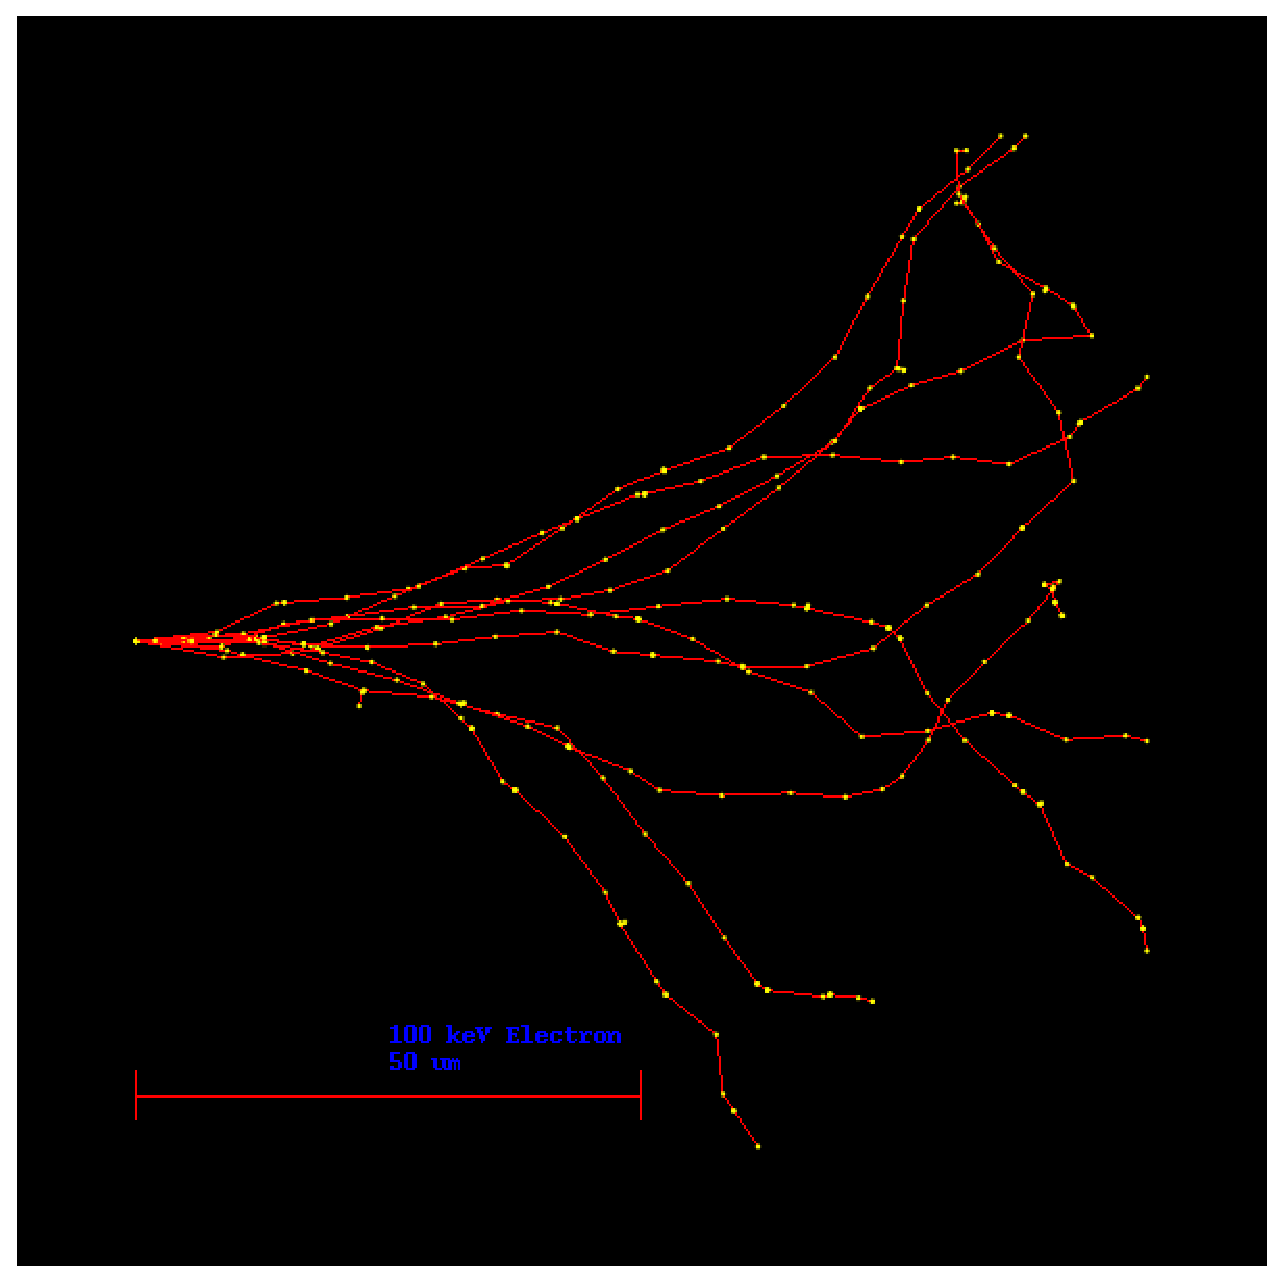
\includegraphics[width=\textwidth]{electronTrack_100keV_0}
      \caption{\SI{100}{\keV} Electron}
    \end{subfigure}
   ~ 
    \begin{subfigure}[b]{0.45\textwidth}
      \includegraphics[width=\textwidth]{electronTrack_50keV_0}
      \caption{\SI{50}{\keV} Electron}
    \end{subfigure}%
    \caption{GEANT4 simulated Particles tracks of a \SI{10}{\keV} electron, \SI{100}{\keV} electron}
  \end{figure}
\hyperlink{EDepScint}{\beamerbutton{Return to Scintillation}}
\hyperlink{toc}{\beamerbutton{Table of Contents}}
\end{frame}
%%%%%%%%%%%%%%%%%%%%%%%%%%%%%%%%%%%%%%%%%%%%%%%%%%%%%%%%%%%%%%%%%%%%%%%%%%
\begin{frame}{Pulse Height Deficits}
\begin{table}
    \caption[Simulated Number of Optical Photons for Selected Neutron Absorptions]{GEANT4 simulated number of optical photons produced for the \iso[10]{B} and \iso[6]{Li} neutron absorptions.  The scintillator is assumed to have a light yield of 1,000 photons per MeV}
    \small
    \centering
    \begin{tabular}{c c c | c}
      \toprule
      & Particle & Photons Produced & Pulse Height Deficit \\
      \midrule
      \multirow{3}{*}{\iso[10]{B}} & $\alpha$ (\SI{1.78}{\MeV}) & 72 $\pm$ 8 &  \\
      & \iso[7]{Li} (\SI{1.02}{\MeV}) & 42 $\pm$ 8 & 27 \\
      & electron (\SI{2.78}{\MeV}) & 3,030 $\pm$ 160 & \\
      \hline
      \multirow{3}{*}{\iso[6]{Li}} & $\alpha$ (\SI{2.05}{\MeV}) & 87 $\pm$ 9 & \\
      & triton (\SI{2.75}{\MeV}) & 528 $\pm$ 23 & 8.5\\
      & electron (\SI{4.78}{\MeV}) & 5,250 $\pm$ 300 & \\
      \bottomrule
    \end{tabular}
  \end{table}
\hyperlink{EDepScint}{\beamerbutton{Return to Scintillation}}
\hyperlink{toc}{\beamerbutton{Table of Contents}}
\end{frame}
%%%%%%%%%%%%%%%%%%%%%%%%%%%%%%%%%%%%%%%%%%%%%%%%%%%%%%%%%%%%%%%%%%%%%%%%%%
